

\section{Background}\label{section:background}
In this section, we first introduce CHCs and explain why program verification can be encoded to CHCs.
%
Secondly, we introduce one of the main streams to solve CHCs by using CEGAR and predicate abstraction.
%
Finally we introduce two mian components (i.e., representing CHCs by graphs and \hyperedgeGNN) in CHC-R-HyGNN framework.


\subsection{Encode Program Verification to Horn Clauses}
%% definition of CHC
A CHC can be written in the form
$H \leftarrow B_{1}  \wedge \cdots \wedge B_{n} \wedge \varphi$,
where $B_{i}$ is an application $p_{i}(t_{1}^{i} \cdots, t_{k}^{i})$ of an uninterpreted fixed-arity relation symbol $p$ to a list of first-order terms;
 $H$ is either an application $p(t_{1} \cdots, t_{k})$, or $\mathit{false}$;
 $\varphi$ is a constraint over some background theory.
Here, $H$ and $B_{1} \wedge \cdots \wedge B_{n} \wedge \varphi$ in the left and right hand side of implication $\leftarrow$ are called ``head" and ``body", respectively.
%
The first-order variables in a CHC are implicitly universally quantified.

%%

CHCs can naturally encode the program verification problem since a CHC can express 
\begin{inparaenum}[(i)]
  \item an assumption by $p_{0}(\bar{t})\leftarrow Assume(\bar{t})$, where $Assume(\bar{t})$ is a first-order formula encoding the assumption condition at control location $0$ over a vector of variables $\bar{t}=(t_{1}^{0},\cdots,t_{k}^{0})$;
  \item A Floyd-style inductiveness condition by $p_{i}(\bar{t}) \leftarrow p_{i^{'}}(\bar{t^{'}}) \wedge T(\bar{t},\bar{t^{'}})$, where $T(\bar{t},\bar{t^{'}})$ is a first order formula encoding the transition condition between the control location $i$ and $i'$; or
  \item an assertion by $\textit{false}\leftarrow p_{i}(\bar{t}) \wedge \neg Assertion(\bar{t})$,  where $Assertion(\bar{t})$ is a first-order formula encoding an assertion condition at the control location $i$.
\end{inparaenum}
For instance, the loop body of $while(x\neq 0)\{x=x+1;\}$ can be encoded to $L(x)\leftarrow L'(x') \wedge x'\neq 0 \wedge x=x'-1 $.
%
The program is safe if and only if the encoded CHCs are satisfiable.


\subsection{Solving Horn Clauses with Predicate Abstraction and CEGAR}

CEGAR \cite{10.1007/10722167_15} is one of the state-of-art frameworks for solving model checking problems by iteratively refining the abstract model.
%
The process is shown in Figure \ref{fig:CEGAR}, where it begins from a model's abstraction $\widehat{M}$.
%
If the abstraction is satisfy the property, then the concrete model satisfy the property as well (i.e., the system is safe), otherwise, a counter-example is generated and the feasibility (spuriousness) is checked. If the counter-example is feasible, the model is unsatisfiable to the property (i.e., system error).
%
If the counter-example is infeasible, the abstraction is over-approximated and needs to be refined.
%
The property is checked again with the refined new abstracted model $\widehat{M'}$.

\begin{figure}[t]
\centering
  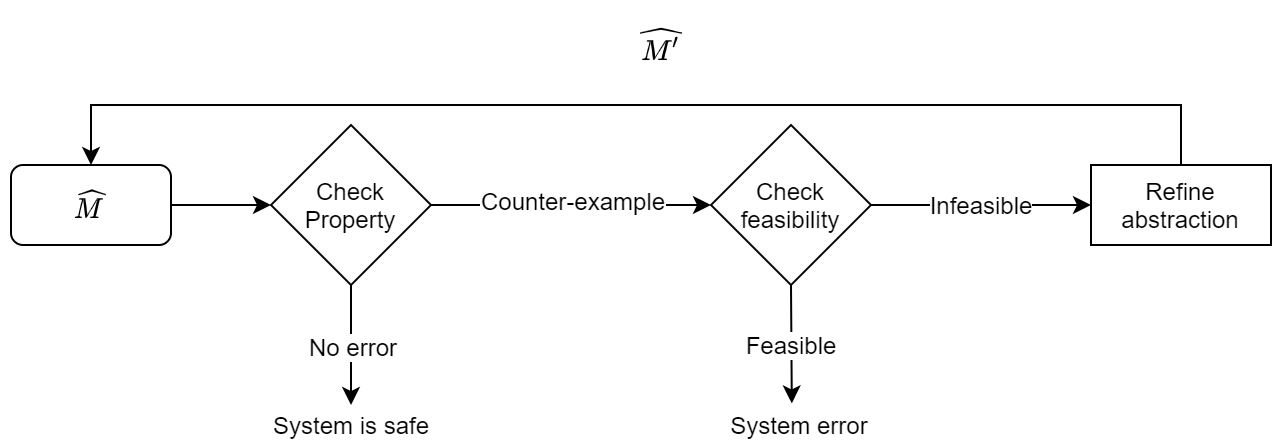
\includegraphics[width=\textwidth]{figures/CEGAR}
  \caption{CEGAR framework.}\label{fig:CEGAR}
\end{figure}

Similar to the CEGAR process, predicate abstraction based model checkers, such as %\cite{10.1145/2254064.2254112} and 
Eldarica~\cite{ruemmer2013disjunctive} construct solutions for CHCs by building an \emph{abstract reachability graph} (ARG) over a set of given predicates. 
%
The solver attempts to construct a closed ARG (check property) from a initial predicate set (abstract model).
%
If a closed ARG is constructed successfully (no error), the CHCs are solvable (system is safe).
%
If it fails to construct a closed ARG, an counter-example (a path from entry clauses to a violated assertion clauses) is extracted.
%
The feasibility is checked by a theorem prover.  If the counter-example is feasible, then the CHCs are unsatisfiable (system error).
%
If the counter-example is infeasible, additional predicates are generated by means of Craig interpolation (refine abstraction).
%to eliminate the spurious counter-examples to be new abstract model






\subsection{Abstract Interpretation with Templates}

An interpolation problem is to finding an interpolant $I$ such that for a conjunction $A\wedge B$, $I\rightarrow A$ and $B\rightarrow \neg I$, where $I$ contains variables that occur in both $A$ and $B$
%
% For an interpolation query $A \wedge B$, an interpolant is a formula $I$ that satisfies \begin{inparaenum}[(i)]
%   \item $A\rightarrow I$;
%   \item $B\rightarrow \neg I$;
%   \item $I$ only contains variables in both $A$ and $B$.
% \end{inparaenum}
Craig interpolation can be used to systematically
refine the abstract model.
%
Guiding the theorem prover to the interpolants containing the suitable predicates in infinite lattice of interpolants is challenging. 
 
%%
 
Abstract interpretation \cite{Leroux2016} is a semantic and solver-independent framework, which modifies the interpolation query for the theorem provers to compute 
possibly user-specified or quantified interpolants that might be hard to find for the prover alone.
%
The framework fist apply an exploration algorithm to search maximal feasible interpolation abstractions in abstract lattice (the powerset of lattice over templates).
%
Then, the maximal feasible interpolation abstractions is used to form the new interpolation query. Constructing  abstraction lattice is essential for systematically explore the infinite interpolant lattice.
%
However, the templates for generating abstraction lattices are selected through static analyses for the program features.
%
In this study we select the templates by automatically learned semantics.


\subsection{CHC-R-HyGNN framework}

\subsubsection{Graph Encoding for Constrained Horn Clauses.}

Graph is a suitable format to represent CHC-encoded problems since they contain rich structural information.
%
We represent the CHCs by two graphs with typed nodes and edges (i.e., \emph{control- and data-flow hypergraph} (CDHG) and \emph{constraint graph} (CG)) to emphasis syntactic and semantic information \cite{HornGraph}.
%
In the Figure \ref{fig:CDHG-CG-examples}, we list concrete examples which represent the CHC $L(x)\leftarrow L(x') \wedge x'\neq 0 \wedge x=x'-1 $ by CDHG and CG.
%
Intuitively, The CG parse CHCs in three different aspects, relation symbol, clause structure, and constraint, to describe the relations between relation symbols and their arguments, abstract syntax of head and body, and constraint.
%
The CDHG draw all symbols in CHCs as typed nodes and use control and data flow hyperedge to describe the control and data flow in verification problems. 

%%

Formally, A graph with typed node and edges, $G=(V,\mathit{E},R,X,\ell)$, consists of a set of nodes $v\in V$, a set of typed edges $\mathit{E} \in V^{*} \times R$ where $V^{*}$ is a list of node from $V$, a set of node types $x\in X$, a set of edge types $r\in R$, and a map $\ell: v\rightarrow x$.
%
The detailed constructing process from CHCs to CG and CDHG is in \cite{HornGraph}.


\begin{figure}[t]
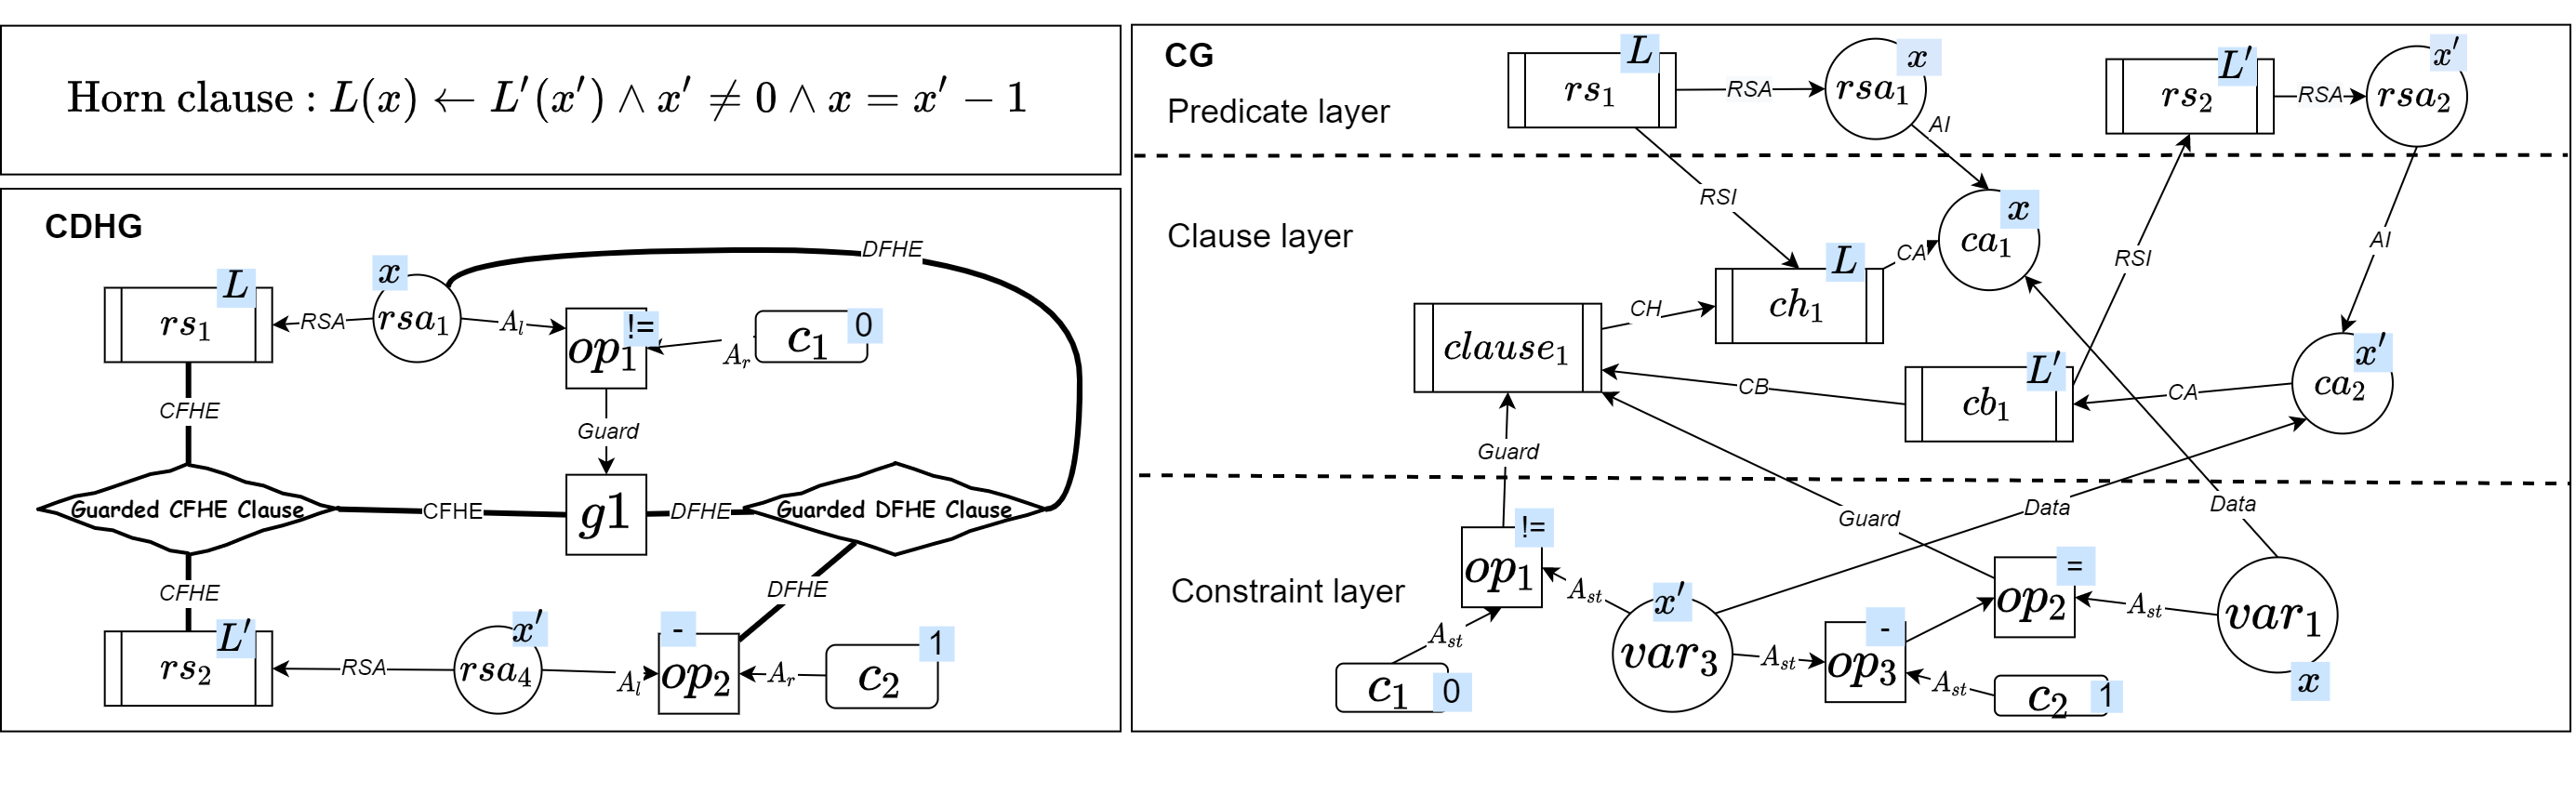
\includegraphics[width=\textwidth]{figures/CDHG-CG-examples.png}
\caption{CDHG and CG} \label{fig:CDHG-CG-examples}
\end{figure}


\subsubsection{Relational Hypergraph Neural Network (\hyperedgeGNN).}

% Message passing-based GNNs are powerful tools for learning features from problems with graph representations.
% %
% It assumes a node can capture local structural information from $t$-hop's neighbors through updating the node representation using aggregated neighbors' representations. Formally, the node representation at timestep $t$ can be computed by
% \begin{equation}\label{message-passing-based-GNN}
%   h_{v}^{t} = \phi(\rho(\{h_{u}^{t-1}|u \in N_{v}^{r}\}), h_{v}^{t-1}),
% \end{equation}
% where $\phi$ and $\rho$ are update and aggregate function, respectively, and
% $N_{v}^{r}$ is $v$'s neighbor nodes in edge type $r$.

% %%

Since CDHG is hypergraph (a graph with edges which connect arbitrary number of nodes), we choose a more generalized MP-GNN architecture \hyperedgeGNN to learn the features.
The node representation updating rule for \hyperedgeGNN at time step $t$ is
\begin{equation}\label{eq:hyperedge-GNN-definition}
  h_{v}^{t} = {\rm ReLU}(\sum_{r\in R}\sum_{p\in P_{r}}
  \sum_{e \in E_v^{r,p}}
  W_{r,p}^{t}\cdot \| [ h_{u}^{t-1}\mid u\in e ] ),
\end{equation}


where $\| \{\cdot \}$ means concatenation of all elements in a set, 
$r \in R = \{ r_i \mid i \in \mathbb{N} \}$ is the set of edge types (relations), 
$p \in P_{r} = \{ p_{j} \mid j\in \mathbb{N} \}$ is the set of node positions under edge type $r$,
$W_{r,p}^{t}$ denotes learnable parameters when the node is in the $p$th position with edge type $r$, and  $e\in E_v^{r,p}$ is the set of hyperedges of type $r$ in the graph in which node $v$ appears in position $p$, where
$e$ is a list of nodes.
The initial node representation $h_{v}^{0}$ is derived from the node types. Note that \hyperedgeGNN can handle multiple edge types with the same number of connoted nodes. For instance, It can handle CDHG which consists of five binary and two ternary edges.




